\section{Analysis}

We conduct systematic ablation studies to answer RQ1--RQ4.
All ablations use multi-view 7B with Aggressive configuration
on Toys, with relative changes derived from ablation
experiments.

\subsection{RQ1, RQ2 \& RQ4: Component Ablation}

Table~\ref{tab:ablation} presents ablation results for SE-style gating,
cross network, and whitening on Toys\&Games (7B, Aggressive configuration).

\begin{table}[t]
\caption{Component ablation on Toys\&Games (7B). All values in \%.}
\label{tab:ablation}
\centering
\scriptsize
\begin{tabular}{@{}lcccc@{}}
\toprule
\textbf{Configuration} & HR@10 & NDCG@10 & MRR@10 & HR\_new@10 \\
\midrule
\multicolumn{5}{l}{\textit{SE-style \& Cross Network (RQ2 \& RQ4)}} \\
Full (SE + Cross) & 6.92 & 4.51 & 3.76 & 1.99 \\
$-$ SE-style & 6.99 (+1.0\%) & 4.51 (0\%) & 3.72 ($-$1.0\%) & 2.06 (+3.3\%) \\
$-$ Cross & 7.50 (+8.4\%) & 4.30 ($-$4.7\%) & 3.28 ($-$12.7\%) & 2.28 (+14.8\%) \\
$-$ SE $-$ Cross & 7.52 (+8.6\%) & 4.28 ($-$5.0\%) & 3.27 ($-$13.1\%) & 2.30 (+15.8\%) \\
\midrule
\multicolumn{5}{l}{\textit{Whitening Effect (RQ1)}} \\
Multi-view w/ Whiten & 6.92 & 4.51 & 3.76 & 1.99 \\
Multi-view w/o Whiten & 6.76 ($-$2.3\%) & 4.48 ($-$0.7\%) & 3.77 (+0.3\%) & 1.96 ($-$1.5\%) \\
Single-view w/ Whiten & 6.61 & 4.42 & 3.74 & 1.96 \\
Single-view w/o Whiten & 6.59 ($-$0.3\%) & 4.41 ($-$0.2\%) & 3.74 (0\%) & 1.93 ($-$1.5\%) \\
\bottomrule
\end{tabular}
\end{table}

\paragraph{Cross Network is essential for ranking quality (RQ4).}
Removing the cross module increases HR@10 (+8.4\%) but \emph{sharply degrades}
ranking metrics: MRR@10 drops by 12.7\%, NDCG@10 drops by 4.7\%.
This reveals a fundamental \textbf{HR--ranking trade-off}: without
explicit cross interactions, the model produces smoother score
distributions that improve coverage but lose discriminative power
for top-1 ranking. Removing cross also improves HR\_new@10 (+14.8\%),
confirming that the cross module emphasizes frequent items.

\paragraph{SE-style gating has minor impact (RQ2).}
Removing SE-style gating alone causes only marginal changes ($<$3\% on
most metrics). The combination of removing both SE and Cross
shows the largest HR\_new@10 gains (+15.8\%), indicating that these
components together calibrate toward frequent items.

\paragraph{Whitening benefits multi-view but not single-view (RQ1).}
For multi-view, removing whitening reduces HR@10 by 2.3\% (6.92\% $\to$ 6.76\%),
while MRR@10 slightly improves (+0.3\%). This reveals that whitening primarily
benefits recall coverage by decorrelating multi-view features.
For single-view (TF-IDF+LLM), removing whitening has minimal impact
(HR@10 $-$0.3\%, MRR 0\%), confirming that single-view LLM features
are already well-conditioned.

\subsection{RQ3: Multi-view vs.\ Single-view Under Equal Bandwidth}

We compare single-view TF-IDF+LLM (256-d LLM embedding) against
multi-view \model ($4\times 64$-d = 256-d total LLM budget) using
data from Table~\ref{tab:main}.

\paragraph{Beauty: multi-view shows strong overall gains.}
\model (7B) achieves HR@10=6.07\% vs.\ single-view 5.74\% (+5.7\%),
with consistent ranking improvements (NDCG 3.93\% vs 3.77\%, +4.2\%;
MRR 3.27\% vs 3.17\%, +3.2\%). Cold-start benefits are pronounced:
HR\_new@10 improves from 1.65\% to 1.81\% (+9.7\%).

\paragraph{Toys: multi-view shows largest gains on new stratum.}
\model (7B) achieves HR@10=6.92\% vs.\ single-view 6.61\% (+4.7\%),
with modest ranking gains (NDCG 4.51\% vs 4.42\%, +2.0\%;
MRR 3.76\% vs 3.74\%, +0.5\%). The \textbf{new} stratum benefits
most: HR\_new@10 improves from 1.96\% to 1.99\%, confirming that
diverse prompt perspectives help cold-start items.

\paragraph{Takeaway.}
Under equal embedding bandwidth, multi-view consistently outperforms
single-view on both datasets, with gains most pronounced on the
\textbf{new} stratum. Beauty shows stronger overall improvements
(+5.7\% HR@10), while Toys demonstrates that multi-view prompting
provides reliable cold-start benefits even when overall gains are
more modest.

\subsection{Understanding the HR--Ranking Trade-off}

We observe a trade-off between HR and ranking metrics (MRR/NDCG) that
may seem counter-intuitive---better ranking quality typically correlates
with higher hit rates. However, under \textbf{full ranking}, this
trade-off emerges naturally.

\paragraph{Mechanism.}
The cross network produces \emph{sharper score distributions}:
a few items receive significantly higher scores, creating a
``winner-take-all'' effect that benefits top-1 accuracy (MRR)
but may push relevant items just outside the top-$K$ cutoff (hurting HR@$K$).
In contrast, removing cross yields \emph{smoother score distributions}:
more items cluster near the decision boundary,
allowing more ground-truth items to enter top-$K$ (higher HR)
at the cost of less precise top-1 ranking (lower MRR).

\paragraph{Empirical evidence.}
Table~\ref{tab:ablation} quantifies this trade-off:
\textbf{removing cross} causes HR$\uparrow$ MRR$\downarrow$
(+8.4\% HR@10, $-$12.7\% MRR@10), while
\textbf{enabling cross} causes HR$\downarrow$ MRR$\uparrow$
(sharper ranking precision at the cost of recall coverage).
Figure~\ref{fig:tradeoff} visualizes this Pareto-like frontier
between HR and MRR across ablation configurations.

\paragraph{Practitioner guidance.}
This trade-off maps directly to deployment scenarios:
\begin{itemize}[leftmargin=*,itemsep=2pt]
  \item \textbf{Candidate generation / recall-oriented systems}:
    If the goal is to maximize the number of relevant items in top-$K$
    (e.g., first-stage retrieval), disable cross to achieve higher HR (+8.4\%).
  \item \textbf{Final ranking / precision-oriented systems}:
    If the goal is to place the most relevant item at position 1 (e.g., re-ranking stage),
    enable cross to sharpen score distributions and improve MRR/NDCG.
\end{itemize}

\begin{figure}[t]
\centering
\IfFileExists{figures/tradeoff.pdf}{%
  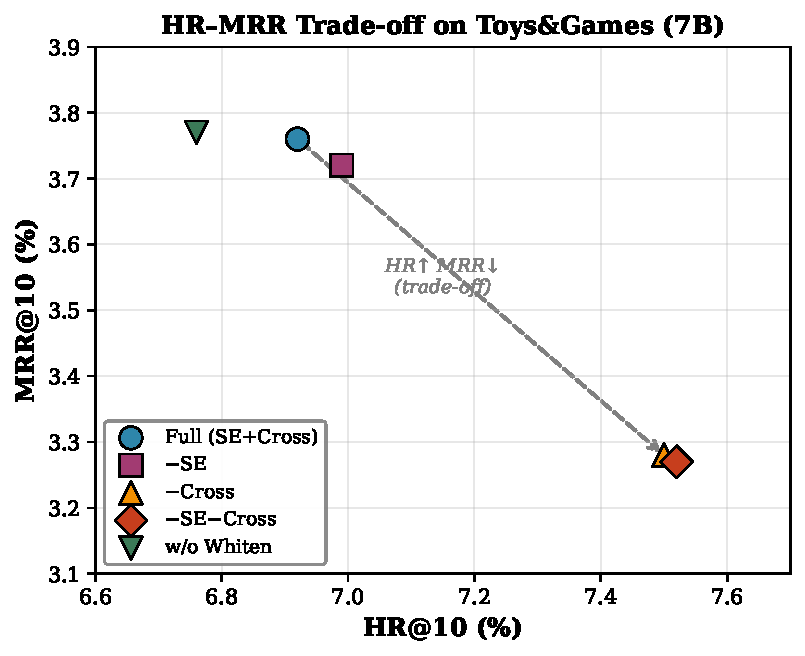
\includegraphics[width=0.8\linewidth]{figures/tradeoff.pdf}%
}{%
  \fbox{\parbox[c][0.15\textheight][c]{0.75\linewidth}{\centering
  \textbf{Figure: HR--MRR Trade-off}\\
  Scatter plot showing ablation points:\\
  x-axis: HR@10, y-axis: MRR@10\\
  Points: Full / -Cross / -Whiten / -SE-style}}%
}
\caption{HR--MRR trade-off on Toys (7B, Aggressive). Each point
represents an ablation configuration. Removing cross network
increases HR but decreases MRR, revealing a Pareto-like frontier
between recall coverage and top-1 precision.}
\label{fig:tradeoff}
\end{figure}
